\documentclass{article}

\usepackage{graphicx}
\usepackage{tikz}
\usepackage{tikzsymbols}
\usetikzlibrary{calc,patterns,shapes.geometric}
\pagestyle{empty}
\usepackage[margin=0pt]{geometry}
\geometry{papersize={14in,12in}}

\def\centerarc[#1](#2)(#3:#4:#5){\draw[#1] ($(#2)+({#5*cos(#3)},{#5*sin(#3)})$) arc (#3:#4:#5);}

\begin{document}
	\begin{figure}
		\centering
		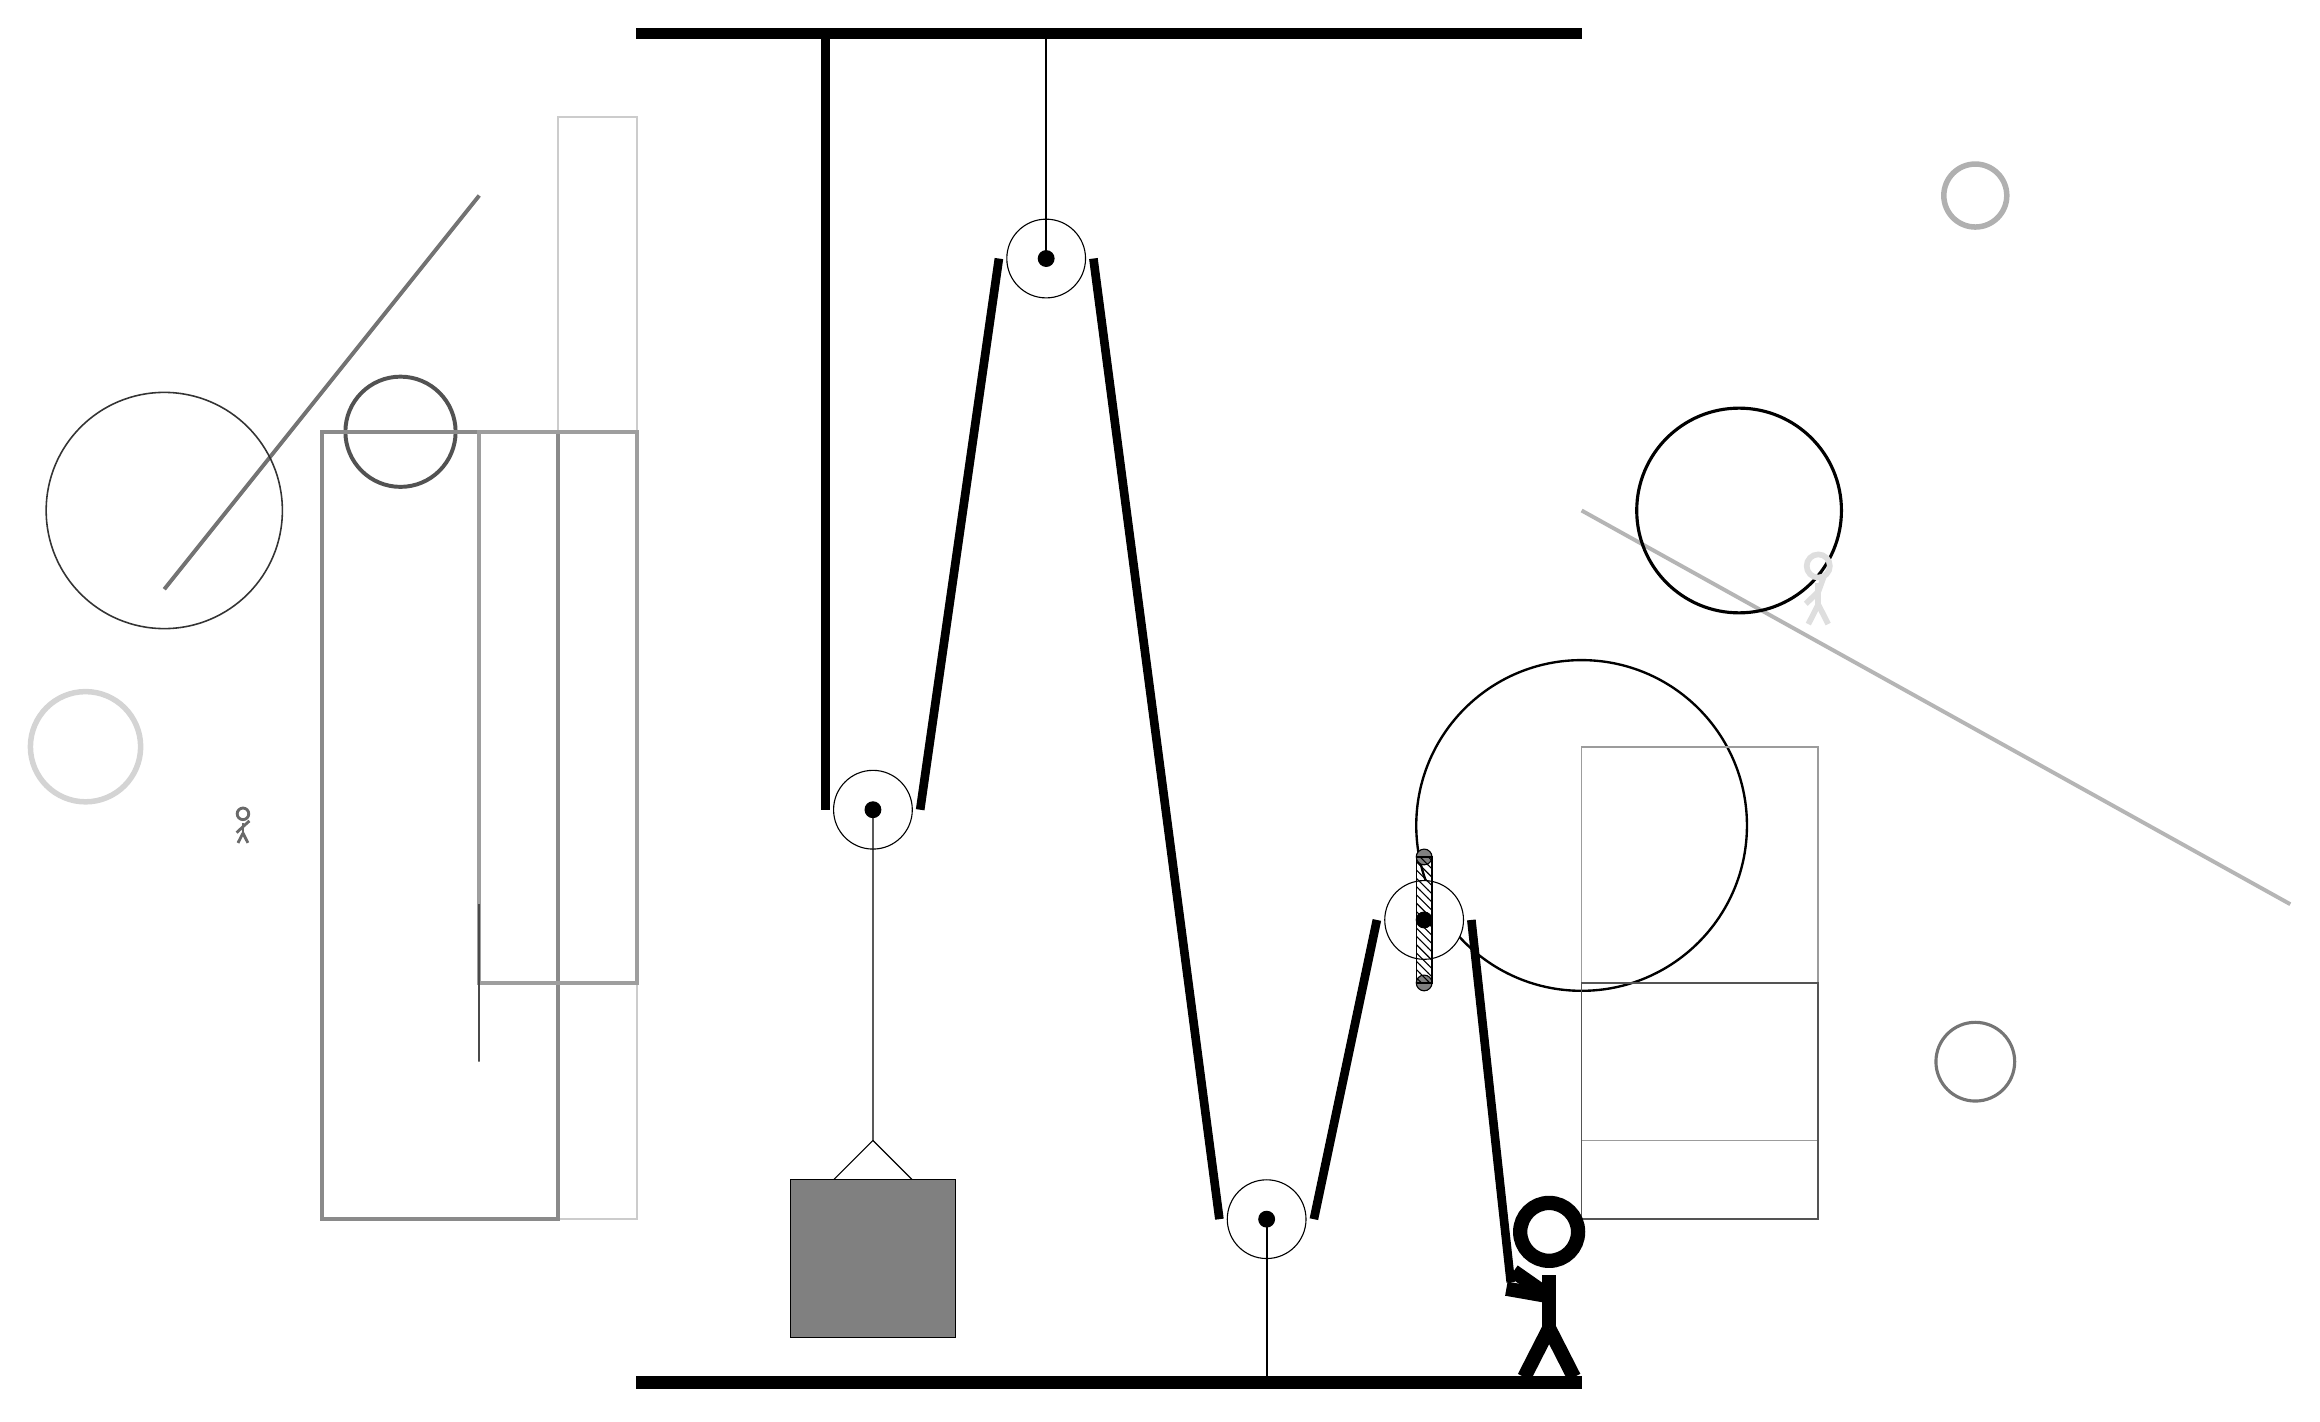
\begin{tikzpicture}
			%%%%% START %%%%%
			
			\draw[fill=black] (-2, 14) rectangle (10, 14.125);
			
			\draw (1, 4.2) circle (0.5);
			\draw[fill=black] (1, 4.2) circle (0.1);
			
			\draw (3.2, 11.2) circle (0.5);
			\draw[fill=black] (3.2, 11.2) circle (0.1);
			\draw[thick] (3.2, 11.2) -- (3.2, 14);
			
			\draw[line width=0.5mm, color=black!29](10, 8) -- (19, 3);
			
			\draw [line width=0.3mm, color=black!100](10, 4) circle (2.1);
			\draw [line width=0.4mm, color=black!54](15, 1) circle (0.5);
			\draw [line width=0.4mm, color=black!100](12, 8) circle (1.3);
			\draw[line width=0.5mm, color=black!55](-4, 12) -- (-8, 7);
			\draw [line width=0.7mm, color=black!31](15, 12) circle (0.4);
			
			\draw[line width=0.3mm, color=black!71] (-3, 9) rectangle (-2, 13);
			\node[line width=0.3mm, color=black!59] at (-7, 4) {\Strichmaxerl[2][43][42]};
			\node[line width=0.7mm, color=black!13] at (13, 7) {\Strichmaxerl[4][44][70]};
			
			\draw [line width=0.5mm, color=black!68](-5, 9) circle (0.7);
			\draw[line width=0.2mm, color=black!20] (-2, 13) rectangle (-3, -1);
			\draw[line width=0.5mm, color=black!46] (-3, -1) rectangle (-6, 9);
			\draw [line width=0.7mm, color=black!17](-9, 5) circle (0.7);
			
			\draw[line width=0.2mm, color=black!39] (10, 0) rectangle (13, 5);
			\draw [line width=0.2mm, color=black!80](-8, 8) circle (1.5);
			\draw[line width=0.5mm, color=black!38] (-2, 2) rectangle (-4, 9);
			\draw[line width=0.2mm, color=black!67] (10, 2) rectangle (13, -1);
			
			\draw[line width=0.3mm, color=black!71] (-4, 3) rectangle (-4, 1);
			
			\draw (6, -1) circle (0.5);
			\draw[fill=black] (6, -1) circle (0.1);
			\draw[thick] (6, -1) -- (6, -3);
			
			\draw[fill=white](8, 2.8) circle (0.5);
			\draw[fill=black] (8, 2.8) circle (0.1);
			\draw[fill=black!50] (8, 3.6) circle (0.1);
			\draw[fill=black!50] (8, 2.0) circle (0.1);
			\draw[pattern=north west lines, pattern color=black] (7.9, 3.6) rectangle (8.1, 2.0);
			
			\draw (1, 4.2) -- (1, 0) -- (0.5, -0.5);
			\draw (1, 0) -- (1.5, -0.5);
			\draw[fill=black!50] (-0.05, -0.5) rectangle (2.05, -2.5);
			
			\draw[line width=1.1mm] (0.4, 14) -- (0.4, 4.2);
			\centerarc[line width=1.1mm](1, 4.2)(180:360:0.6);
			\draw[line width=1.1mm](1.6, 4.2) -- (2.6, 11.2);
			\centerarc[line width=1.1mm](3.2, 11.2)(0:180:0.6);
			\draw[line width=1.1mm](3.8, 11.2) -- (5.4, -1);
			\centerarc[line width=1.1mm](6, -1)(180:360:0.6);
			\draw[line width=1.1mm](6.6, -1) -- (7.4, 2.8);
			\centerarc[line width=1.1mm](8, 2.8)(0:180:0.6);
			\draw[line width=1.1mm](8.6, 2.8) -- (9.1, -1.8);
			
			\node at (9.5, -1.9) {\Strichmaxerl[10][-35][170]};
			
			\draw[fill=black] (-2, -3) rectangle (10, -3.15);
			
			%%%%% END %%%%%
		\end{tikzpicture}
	\end{figure}	
\end{document}